\title{Global Illumination through Atmospheric Scattering}
\author {
  Jonathan Keith Simmons
}
\date{\today}
\documentclass[12pt, letterpaper]{article}
\usepackage{setspace}
\usepackage[margin=1in]{geometry}
\usepackage{graphicx}
\usepackage{amsmath}

\begin{document}
\singlespacing
\maketitle
\doublespacing

\begin{center}
  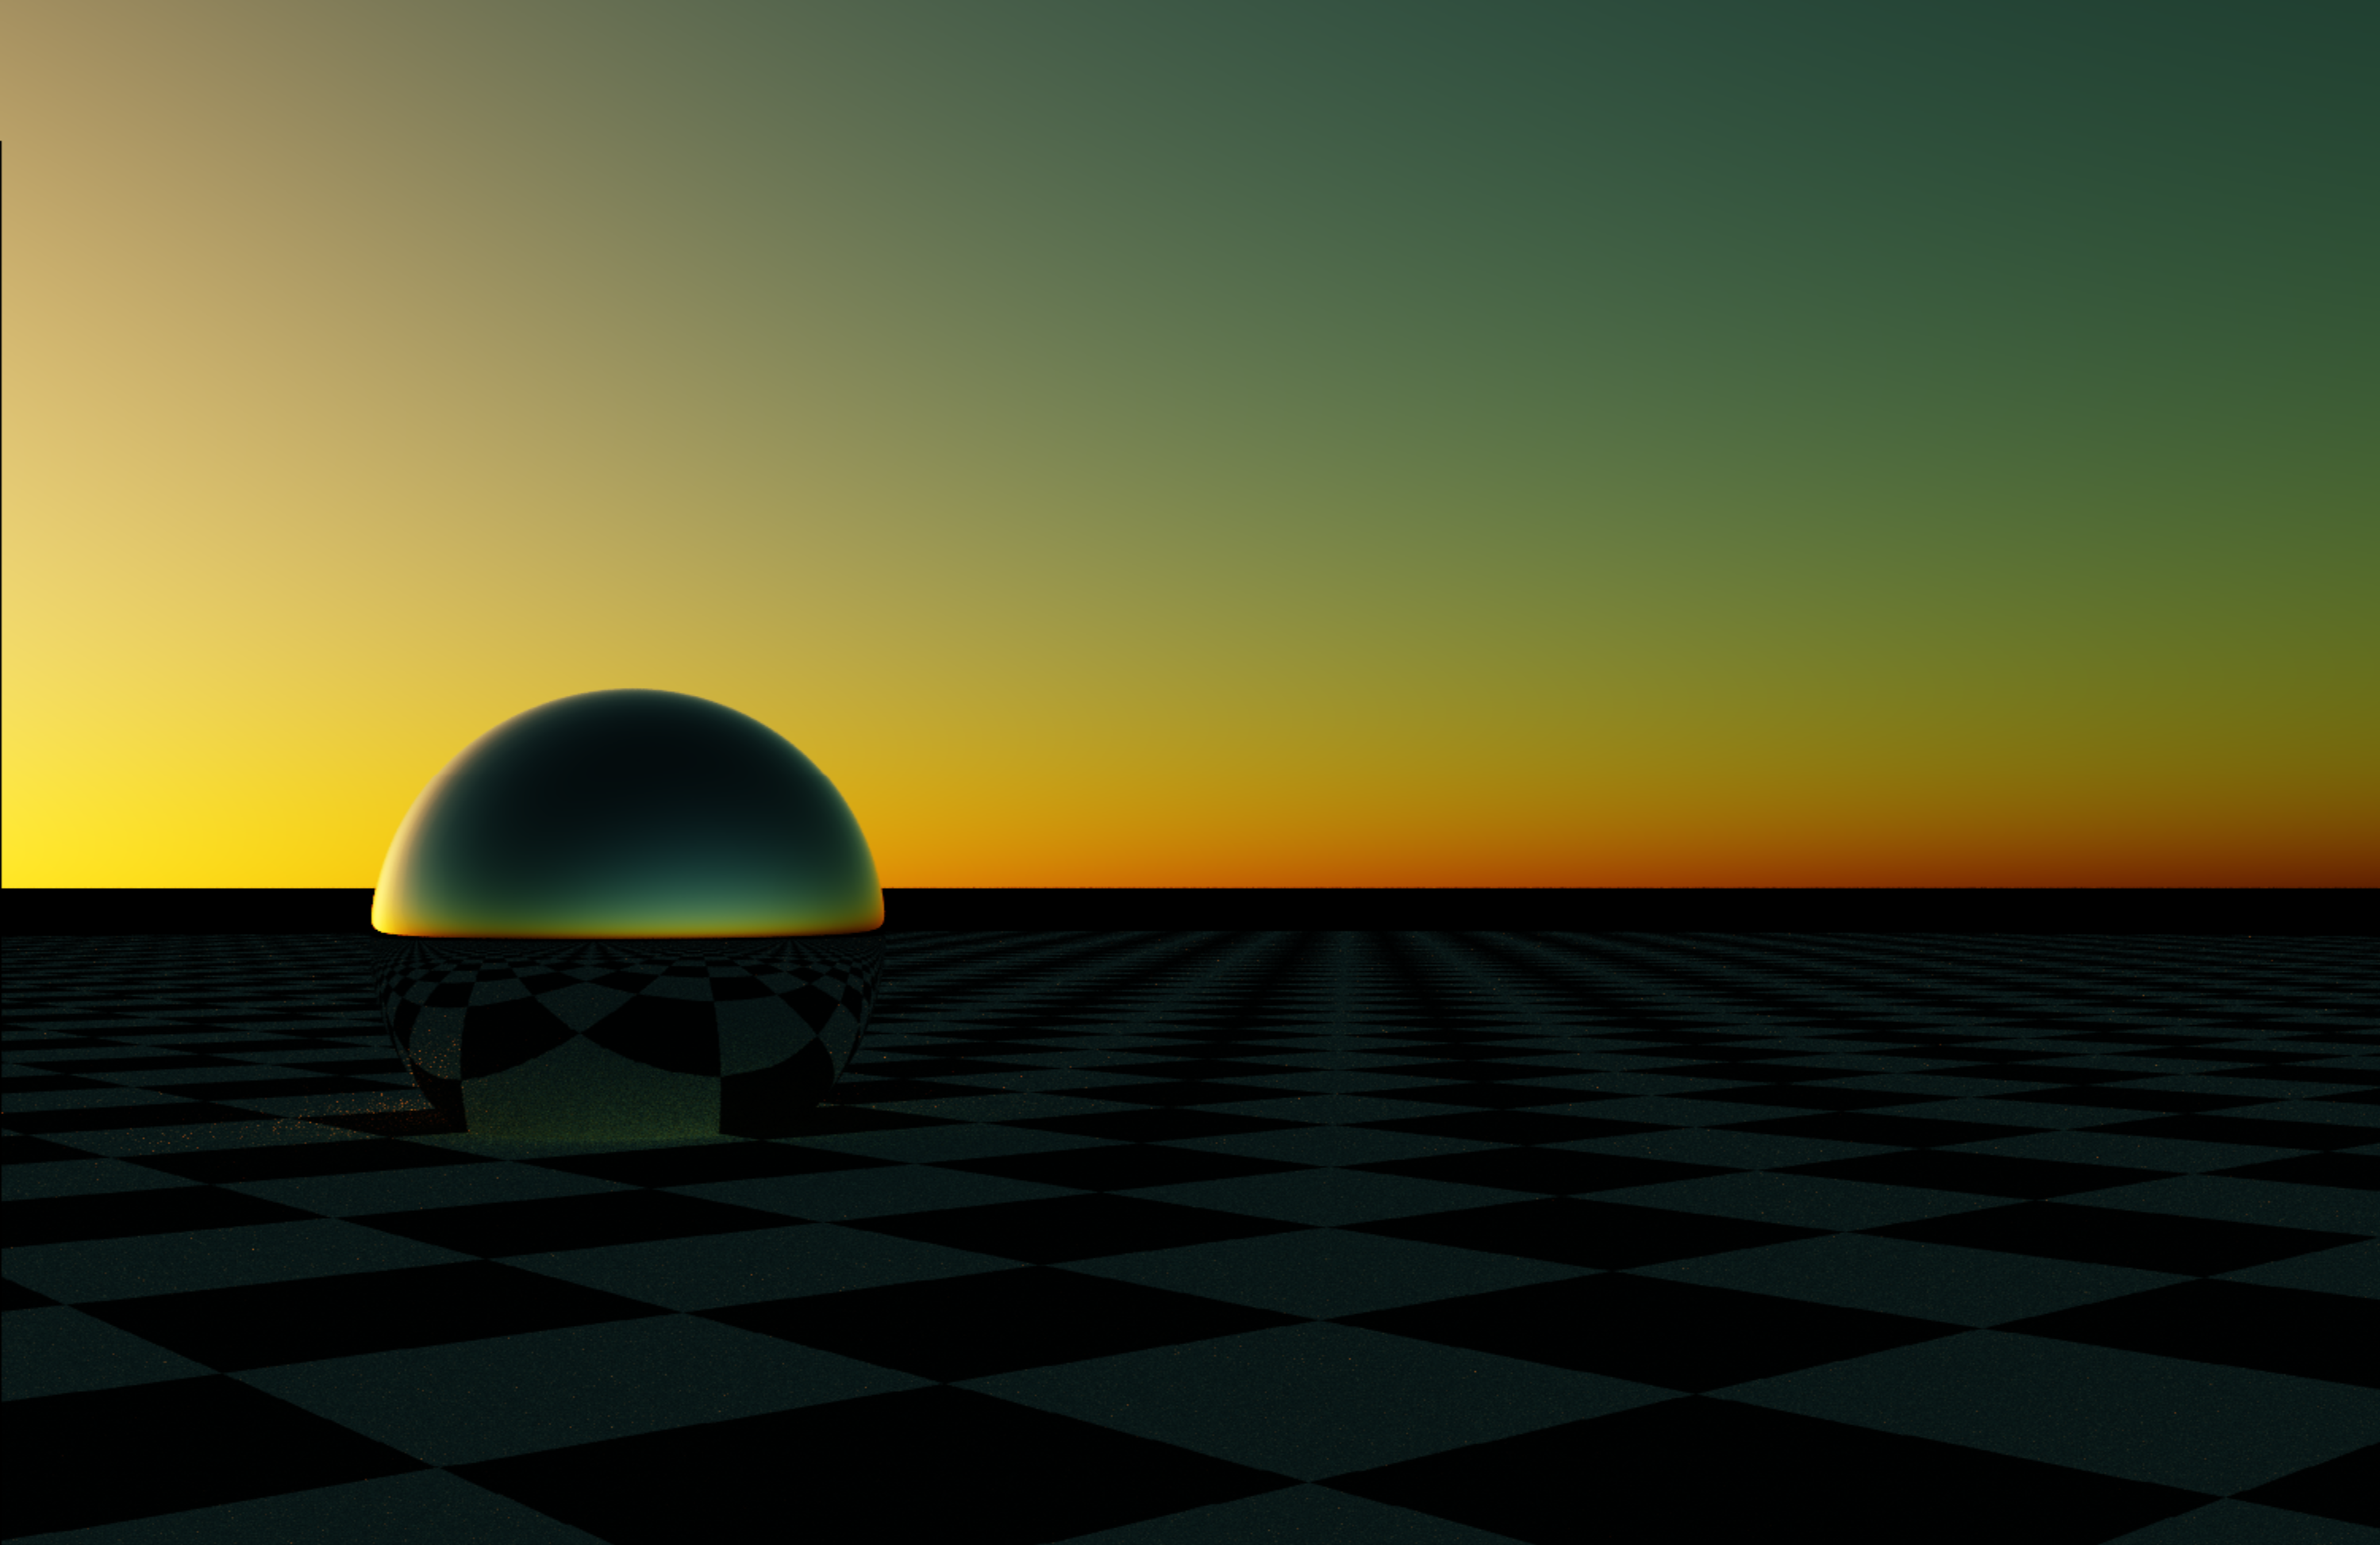
\includegraphics[width=0.8\textwidth]{SunsetSky}
\end{center}

\section{Abstract}

This paper tackles the problem of using models of light scattering in the
atmosphere to globally illuminate a scene for path tracing. Due to the reversible
nature of light we are able to trace it backward from the camera into the scene.
After tracing a number of bounces from the camera the light will either fail to
contribute any illumination to the image, or will escape into the sky. From that
point we can approximate the amount of light that will be scattered from the sun
along the escape path. The final image is the average of the light contribution
from each of the rays traced in the scene and scattered by the atmosphere.

I contribute an implementation of this algorithm to generate images that have
accurate atmospheric lighting and complex lighting effects such as ambient
occlusion.

\section{Problem}

The creation of photo-realistic images can be handled in two main ways. First
images can be approximated from meshes. This method involves deconstructing
objects into triangles which can be transposed and projected onto the screen.
Then the lighting effects for each pixel can be approximated by tracing rays to
relevant light sources and near by objects. The second method involves
simulating light as individual rays which can be tracked through a scene as it
bounces from object to object. The former method is much more optimizable, but
less accurate due to the shortcuts of sending rays toward light sources directly
and representing everything as meshes of triangles.

The second method is incredibly realistic. Light actually travels through space
in straight lines (so long as relativistic effects are ignored) and bounces in
largely predictable distributions. In effect, the amount of light that reaches
each pixel of an image can be modeled as an integral over all of the paths which
enter at that point from a given direction. Unfortunately the integrals involved
are too complex to handle analytically, so the standard solution is to
approximate them with a Monte Carlo method. However to converge on an image
requires sending millions of rays into the scene and averaging the results for
each one. For a simple scene where the only locations for bouncing light is on
objects in the scene, this can be doable on modern computer hardware, but for
volumetric simulation such as that in an atmospheric model the number of rays
required becomes untenable.

This paper examines the second method for rendering realistic scenes. It
analyzes an efficient method for approximating light travel through an accurate
earth atmosphere by developing extinction coefficients which are sampled at
various heights in the simulated atmosphere. By building a good model for light
that scatters from the sky. I can adapt the model for global illumination of a
scene which produces better and more realistic colors for arbitrary times of day
including the so called ``Magic hour'' and sunsets/sunrises.

Note: This paper does not go into the mechanics of a general path tracer such as
simulation of roughness and reflections. Instead I provide the necessary
background information to understand the addition of accurate atmospheric
lighting and largely ignore the mechanics of rendering the scene portion of the
program. If desired, the code (in the state that its in) can be found at the
github link https://github.com/Kethku/PathTracer.

\section{Simplifications}

A fundamental assumption with Monte Carlo image techniques is that light can be
traced backwards to produce identical images to those produced when traced
forward. This assumption is based on two facts. First is that light will always
bounce symmetrically about the normal of a surface, and second that light can be
assumed to travel in straight lines at all times \cite{veach}. This means that
the same equations can be applied for light going in reverse as to light
traveling forward from light sources. This assumption is useful because the only
light which contributes to the color in the final image is light which entered
the viewport at very specific angles. So instead of simulating random paths from
light sources into the scene, we only need to sample light which leaves the
camera. This yields a huge increase in performance for zero loss in quality.

We can also assume that so long as the scene is small enough we do not need to
simulate the effects of the atmosphere on the light rays local to the scene.
This assumption makes sense in every day experience because light does not often
look hazy (unless particles are in the air effecting things). Due to this fact
we can speed up the calculation further by only simulating atmospheric
scattering after the light has left the scene and just use straight light paths
for interactions with scene objects. This also allows our atmospheric
calculations to ignore obscuring from objects in the scene as any light that
escapes is likely too far from the scene to be effected by it.

In effect we can split the problem of rendering a scene into two portions: the
initial bounces about the scene without atmosphere and the subsequent effects
due to the atmosphere without the scene \cite{scratch}. By ignoring the scene in
the atmospheric calculations, we can calculate light along a given path by
approximating the integral of all the light scattered along that path over the
length of the path. This integral has no discontinuities within the bounds which
means we can use numerical methods to approximate the total sum over the path.
In contrast the scene simulation can converge quicker since the only random
effects are due to how light scatters on objects in the scene instead of
including how the light might scatter in the air.

Papers on the topic of atmospheric scattering state that the majority of the
contribution of light from the sky comes from whats called single scattering
\cite{nishita}. We can therefor ignore contribution along a path into the sky
from other atmospheric bounces and can just take into account how much light
would bounce toward the ray from the sun directly. In a more complete
representation of atmospheric scattering one would need to take into account the
bounces of light in the atmosphere after the first bounce. We mitigate the need
to do so through the use of extinction coefficients which simply reduce the
amount of light that makes it to a destination based on the density of the gas
in the convening space due to scattering and or absorption.

The two types of scattering in the atmosphere from non cloud sources is Rayleigh
and Mie scattering \cite{rainbows}. We can simplify the equations further by
ignoring all other types and just handle those two. This makes sense since they
are the primary sources of the sky color.

Due to the characteristics of computer graphics and screens all color
information is encapsulated in values of red blue and green. Given that none of
the scattering algorithms alter the color of the light that goes into it, we can
model the color attenuation (amount of light in each color range which gets
absorbed or scattered) on a per color channel basis. For the purposes of this
paper's rendering I use 440nm for blue, 550nm for green and 680nm for red's
wavelength. These numbers factor into the scattering equation for Rayleigh
scattering.

Furthermore we assume that the earth is a perfect sphere of size 6360 km and
that the atmosphere is 60 km thicker.

We assume that sunlight reaching earth is for all intents and purposes parallel.
This allows us to treat the sun direction as constant over all of the
calculations and speeds up calculations.

Finally we ignore the effects of relativity and quantum mechanics as they
provide little to know effect on the final image.

\section{Mathematical Model}

Monte Carlo light transport algorithms can be thought of as taking the integral
of all of the light entering a particular point in space. By sampling that
integral over the rectangle covering each pixel in the scene space we can build
up an image to display. As stated previously I will not be examining the math
needed to accurately model a ray of light bouncing through a scene. Instead I
will solely look at the math when a ray of light escapes the scene.

The algorithm gives a ray after it has finished bouncing through the scene and
leaves a certain radius.

\begin{gather*}
  R^{Camera} = \{ Pos, Dir \}
\end{gather*}

We also have the vector representing the direction of the sun which I will refer
to by $S$.

I will use this syntax to refer to the Position and Direction components of rays
in calculations: $R^{Camera}_{Pos}$ and $R^{Camera}_{Dir}$.

The earth and atmosphere can be represented as implicit surfaces with radius
$6360 * 1000 m$ and $6420 * 1000 m$ \cite{scratch} respectively yielding equations:

\begin{gather*}
  Earth: x^2 + y^2 + z^2 = (6360 * 1000)^2 \\
  Atmosphere: x^2 + y^2 + z^2 = (6420 * 1000)^2
\end{gather*}

If we calculate the intersection of $R^{Camera}$ with the sphere representing
the atmosphere we get a line segment $(R^{Camera}_{Pos}, P^{CameraIntersect})$

Similarly at any point $X$ along $R^{Camera}$ we can calculate the intersection
between the ray $(Pos = X, Dir = S)$ and the atmosphere which I will refer to as
$P^{SunIntersect}$.

Rayleigh scattering involves light hitting a particle which is much smaller than
the wavelength of the light. The effects of this scattering can be captured in 3
values. $\beta^R_e$, $\beta^R_s$, and $p$. $\beta^R_e$ and $\beta^R_s$ represent the
extinction and scattering attenuation coefficients for Rayleigh style particles
which indicate the amount of light attenuated or scattered per meter traveled
through the atmosphere. In the case of Rayleigh scattering, the
particles never absorb light and will always scatter. This means that the
$\beta^R_e$ and $\beta^R_s$ coefficients are equal for Rayleigh scattering \cite{nishita}.

\[
  \beta^R_s = \beta^R_e = \frac{8 \pi^3 (n^2 - 1)^2}{3N_0\lambda^4}
\]

Where $n$ is the index of refraction for the air and $N_0$ is the molecular density at
sea level. For the purposes of my calculations I will use precomputed versions
of these values for the 3 wavelengths used in my renderer. This removes the need
to have accurate values for the constants in the equation. I will be using the
values suggested by the scratchapixel article. $33.1 * 10^{-6}$ for blue, $13.5 *
10^{-6}$ for green and $5.8 * 10^{-5}$. I will conveniently refer to these three
values as the vector $\beta^R_e$ or equivalently $\beta^R_s$. The equation for
Mie scattering is much more complicated but does not have a dependence on the
wavelength of the light so I will simply use a precomputed constant value of
$210 * 10^{-5}$.

$p^R$ is the phase function for Rayleigh scattering and represents how much
light gets scattered based on the angle between the light and the viewing angle.

\[
  p^R(\mu) = \frac{3}{4}(1 + \mu^2)
\]

Similarly the phase function $p^M$ for Mie scattering can be computed:

\[
  p^M(\mu, g) = \frac{3(1-g^2)(1+\mu^2)}{8\pi(2 + g^2)(1 + g^2 - 2g\mu)^{\frac{3}{2}}}
\]

Where $\mu$ is the $cos(\theta)$ where $\theta$ is the angle between the
incident light angle and the observation angle and where g is the anisotropy
constant of the medium. This determines how much of the light is scattered
backward and how much is scattered forward. In our case the Rayleigh scattering
is not dependent on the anisotropy, but the Mie is \cite{scratch}.

Finally to adjust the attenuation coefficients for the decrease molecular
density due to height we multiply by a factor of $e^{-\frac{h}{H_0}}$ where
$H_0$ is the molecular density at sea level and $h$ is the current height from
sea level.

Combining the above equations we arrive at the amount of light lost due to
Rayleigh scattering over a certain distance (point $a$ to point $b$) $T$. This
equation is known as the attenuation and is interpreted as the ratio of the
remaining light at the end of the movement from $a$ to $b$ to the amount of
initial light.

\[
  A(a, b) = \int^b_a (\beta^R_e + \beta^M_e) e^{-\frac{h}{H_0}}ds 
\]

We can calculate the transmittance over a given distance by calculating the
attenuation over said distance to find the total attenuation and feeding the
negative of that value to the exponential function. This gives us the percentage
of light remaining after traveling that distance in the medium.

\[
  T(a, b) = e^{-A(a, b)}
\]

Finally we can determine how much light would be scattered in a given direction
at a given point by multiplying the sun intensity (I use a constant of 20, but
this only determines the brightness of the image and can be any value) by the
scattering attenuation coefficients, and the phase functions.

\[
  L(X) = SunIntensity * T(X, P^{SunIntersect}) * (p^R * \beta^R_s + p^M * \beta^M_s)
\]

By calculating the integral of this value over the course of the view path we
can get the total light sent back toward the camera. Finally multiplying this
quantity by the transmittance of the path back toward the view ray origin we can
get the light that actually made it back to the camera instead of being
scattered away.

\[
  C(R) = \int_{R_{Pos}}^{P^{CameraIntersect}}T(R^{Camera}_{Pos},X)L(X)ds
\]


\section{Solution}

The intersection between a ray and an implicitly defined sphere can be
calculated through the use of the quadratic equation by introducing a time
variable. We solve for the time ignoring negative solutions because they appear
behind the ray's starting position. If we have a ray $R$ and implicitly defined
sphere of radius $r$,

\[
  |R_{Pos} + R_{Dir}*t|^2 - r^2 = 0
\]

Solving for $t$ with the quadratic equation yields:

\[
  t = \frac{-2R_{Pos}R_{Dir} \pm \sqrt{(2R_{Pos}R_{Dir})^2-4(R_{Pos}^2-r^2)}}{2}
\]

And simplified:

\[
  t = -R_{Pos}R_{Dir} \pm \sqrt{(R_{Pos}R_{Dir})^2-(R_{Pos}^2-r^2)}
\]

The number of solutions to the above equation is determined by the
$(R_{Pos}R_{Dir})^2-(R_{Pos}^2-r^2)$ term. If it is negative, we know that no
solutions exist. If it is positive we know that two solutions exist. In the
second case we only care about positive solutions to the overall equation. If
neither solution is positive, we are still left with no solution. Otherwise we
pick the smallest non negative solution as the first intersection.

The other complication in the solution for this problem is that of unsolvable
integrals. The domains of the integrals in this problem are non trivial to do by
hand and impossible to do in a reasonable amount of time. So instead of solving
the integrals analytically I found that solving them numerically was much more
efficient for little loss in quality.

This was carried out by summing samples along the domain multiplied by the
intervening distance. For example:

\[
  \int_{R_{Pos}}^{P^{CameraIntersect}}T(R^{Camera}_{Pos}, X)L(X)ds \approx \sum_{Xs}T(R^{Camera}_{Pos}, X)L(X)ds
\]

Where Xs is the list of samples evenly spaced over the domain of the integral
and ds is the total length of the domain divided by the number of samples. I
found a good compromise between speed and accuracy was to take 4 samples for the
transmittance integral and 16 samples for the light gathering integral.

The convergence of the final image was calculated as the simple average of the
intensity values of millions of randomly sampled rays into the scene. The
program was designed to send rays using all available cpus and gradually update
the image in real time. This way I could know when the image had converged or
gone far enough toward completion for my taste.

\section{Results}

\begin{center}
  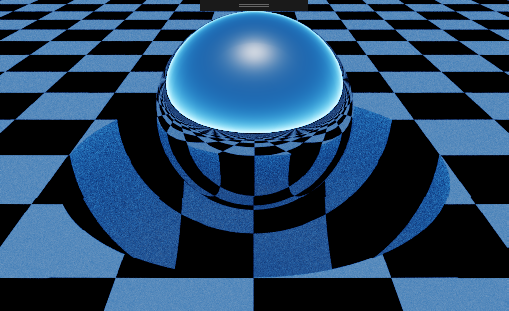
\includegraphics[width=0.45\textwidth]{day}
  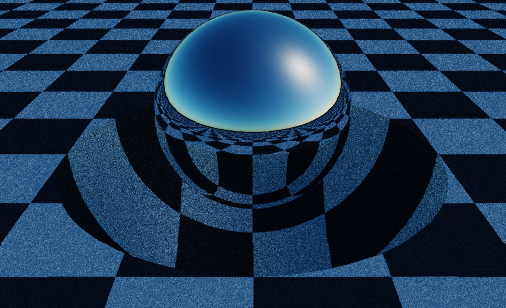
\includegraphics[width=0.45\textwidth]{afternoon}
\end{center}
\begin{center}
  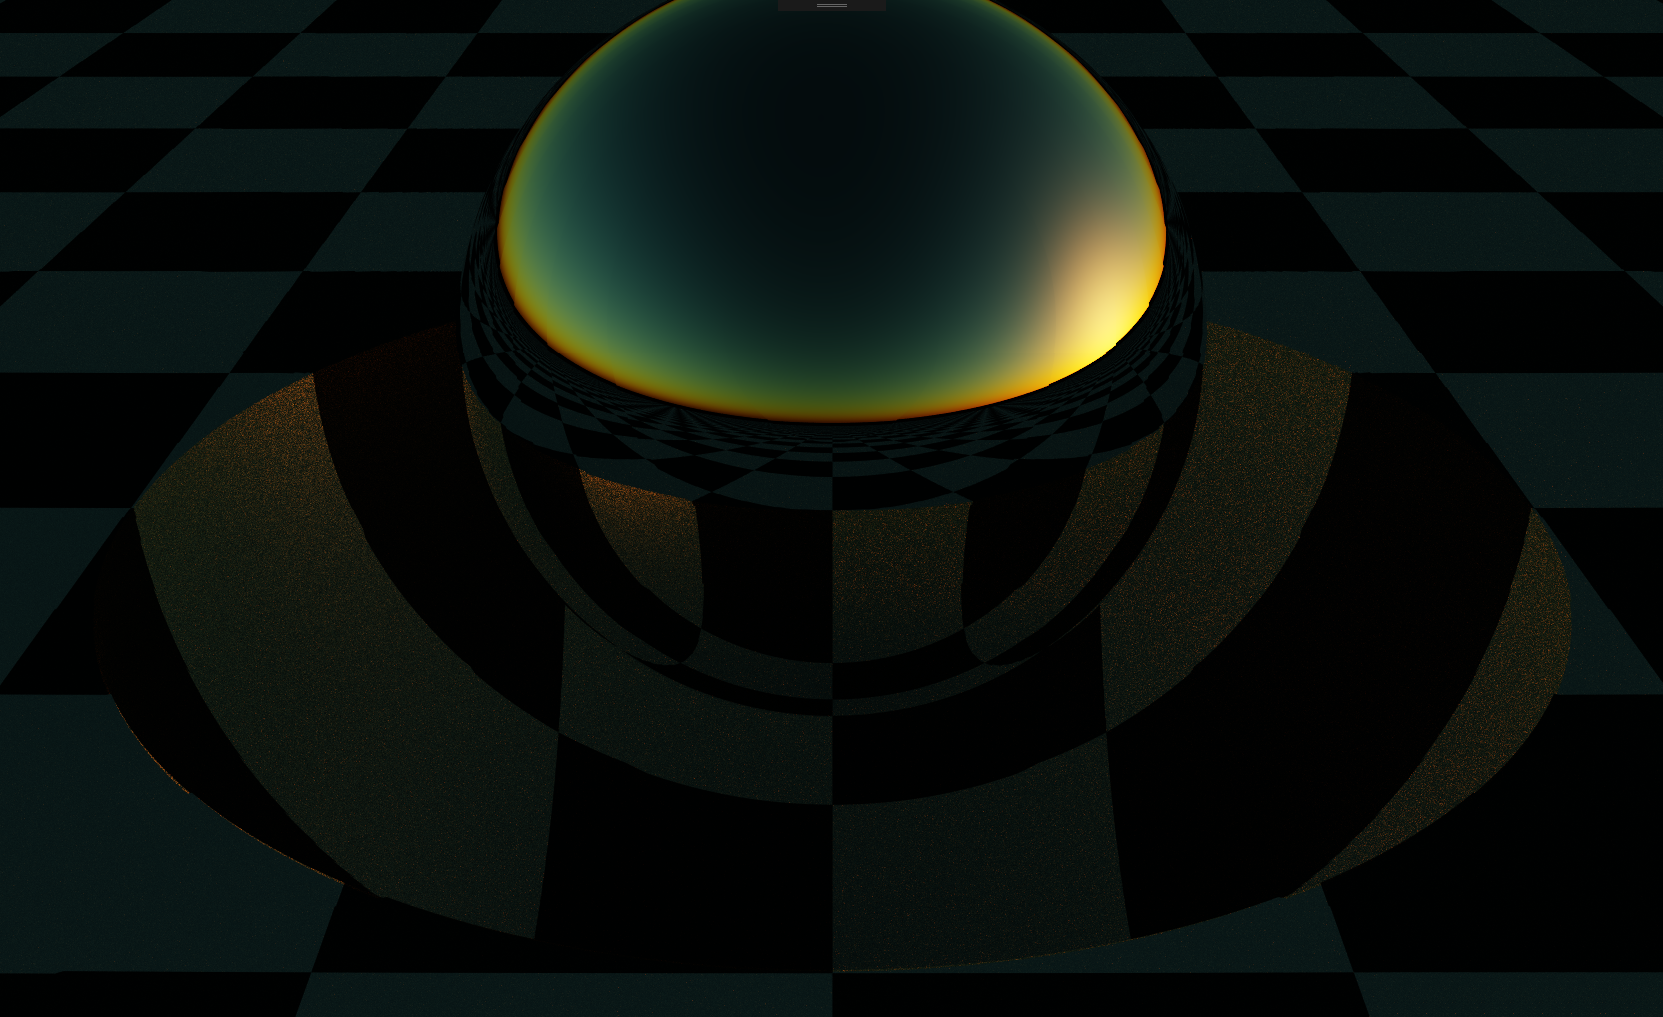
\includegraphics[width=0.45\textwidth]{sunset}
  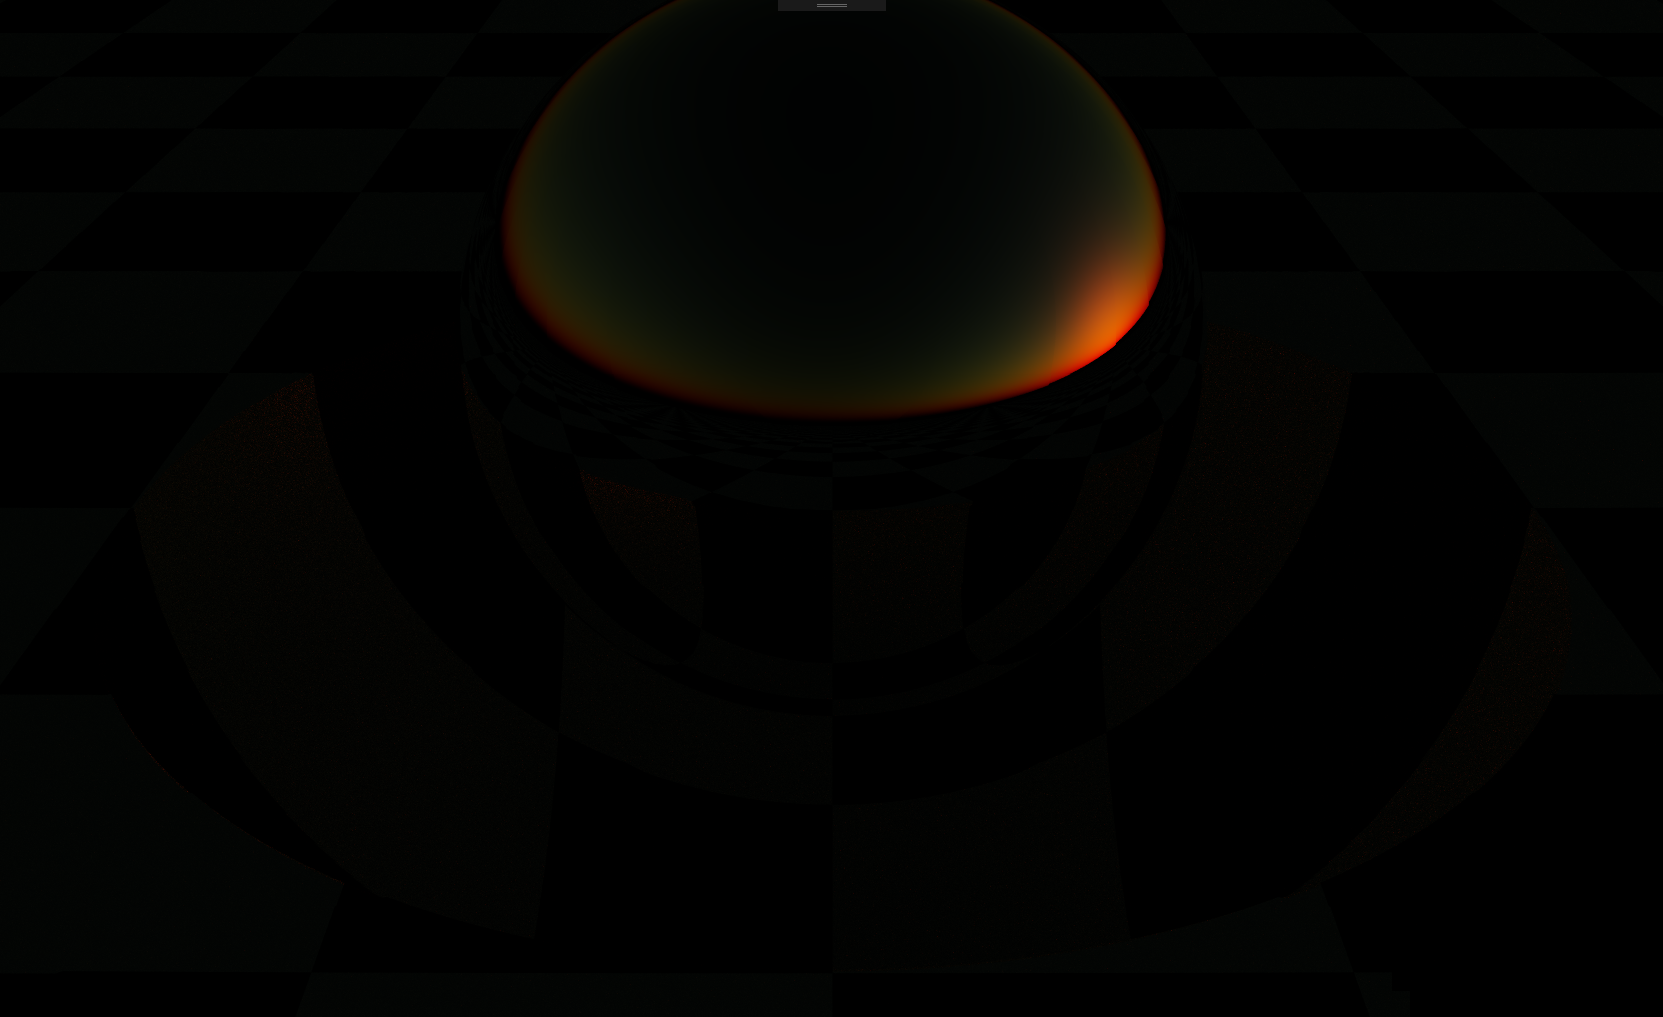
\includegraphics[width=0.45\textwidth]{evening}
\end{center}

The images displayed above are a simple test scene of a matte checkerboard plane with
a hemisphere cut out with a floating completely reflective sphere in the middle
at 4 different sun angles representing noon, afternoon, sunset, and early
evening. This scene was picked in order to highlight the ambient occlusion
properties of the Monte Carlo renderer as well as simple shadows and reflected
light from the sphere.

The results were highly satisfactory and closely mirrored results achieved
in the scratchapixel article and nishita papers. As light travels through the
atmosphere more of the blue light is scattered away. However blue light is
vastly more likely to be scattered toward the camera in the first place. So if
the light does not travel far, it retains the blue tint as expected. The Mie
scattering also contributes to the light from the sky, however given the
independence from wavelength the light contributed is only white.

As the sun gets closer to the horizon, the light must travel farther through the
atmosphere and so more of the blue light is attenuated leaving the red and green
to be transmitted through. We see this effect clearly in the test renders. As
the sun creeps farther down and even past the horizon the sky moves from blue
toward green and red producing the familiar sunset colors.

\begin{center}
  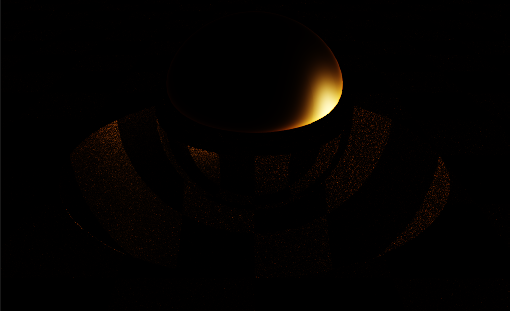
\includegraphics[width=0.45\textwidth]{Occlusion}
  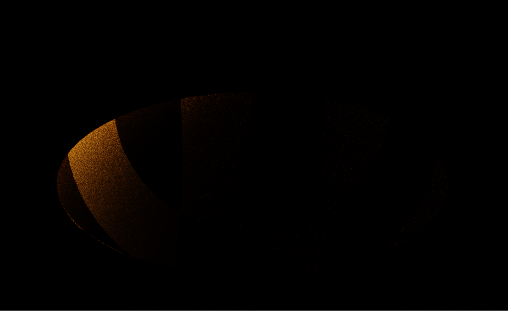
\includegraphics[width=0.45\textwidth]{OcclusionNoSphere}
\end{center}

The above images were rendered at low sun angle and without Rayleigh scattering
to make a sharper light. The left image contains my standard demo scene and the
right contains the same scene but without the reflective sphere in the center.

In these images we can see clearly that light from the sky is accurately bounced
off of the sphere and blocked by the sphere. On the left image we can see
illumination on the right side of the cut out which is absent when the sphere is
not present on the right image. Similarly we can see a shadow cast from the
sphere onto the left side of the divot which is much brighter when the sphere is
not present on the right image.

This type of effect is very difficult to achieve accurately with non Monte Carlo
methods and is still present even with separating the two haves of the
atmospheric lighting equation.

\section{Improvement}

Due to separating the equation into scene calculations and atmosphere
calculations, we do not get lighting effects such as god rays and mist. These
effects require light to scatter multiple times and are much more
computationally intensive. This renderer could be improved by applying similar
techniques to the multi scattering problem.

The renderer could also be greatly improved by porting the code to a fragment
shader on the GPU. Every ray is completely independent from each other which
means that this algorithm is ridiculously parallelizable. The GPU is able to run
100s to 1000s of calculations in parallel instead of the sequential method I use
currently. Even switching to calculating on all available cores is only a
fraction of the speed up that might be possible with the GPU.

Currently my light transport algorithm through the scene is very inefficient. I
send rays into the scene and bounce them without using importance sampling.
Better algorithms have been developed including bidirectional path tracing and
metropolis light transport. It would be interesting to try to adapt those
techniques to a combined atmospheric renderer.

My path tracer also operates on red green and blue values only instead of full
spectrum. As the Rayleigh algorithm effects all wavelengths. I might be able to
achieve more interesting gradients by treating every frequency accurately.

\section{Conclusions}

In this paper I described an efficient approximation of light scattering in an
earth like atmosphere. I discussed the trade offs required to converge on an
accurate image in a realistic amount of time. I built a working renderer using
the techniques described in the paper and provided example images of scenes at
various times to provide evidence toward the accuracy of the model.

\clearpage

\bibliographystyle{unsrt}
\bibliography{references}

\end{document}